%%%%%%%%%%%%%%%%%%%%%%%%%%%%%%%%%%%%%%%%%%%%%%%%%%%%%%%%%%%%%%%%%%%%%%%%%%%%%%%
% Percepatan Inferensi CNN Super-Resolution melalui Reduksi Spasial GPU:
% Studi Lintas Platform pada Arsitektur Memori Terpadu dan Diskret
% Versi bahasa Indonesia dari itis.tex. Seluruh angka, tabel, gambar dan
% referensi identik dengan versi Inggris; hanya prosa yang diterjemahkan.
%%%%%%%%%%%%%%%%%%%%%%%%%%%%%%%%%%%%%%%%%%%%%%%%%%%%%%%%%%%%%%%%%%%%%%%%%%%%%%%

\documentclass[conference]{IEEEtran}
\IEEEoverridecommandlockouts

\usepackage{cite}
\usepackage{amsmath,amssymb}
\usepackage{graphicx}
\usepackage{textcomp}
\usepackage{xcolor}
\usepackage{booktabs}
\usepackage{url}

% IEEEtran menetapkan Courier (pcr) untuk \texttt. Jika paket courier tidak
% terpasang -- ia absen dari skema TeX Live "basic" -- setiap \texttt jatuh ke
% nullfont dan menjadi tidak terlihat sama sekali, hanya dengan peringatan di
% log. Memuatnya secara eksplisit mengubah kegagalan senyap itu jadi error.
% Pasang dengan: tlmgr install courier
\usepackage{courier}

% Istilah Indonesia untuk elemen yang dicetak IEEEtran. Paket babel sengaja
% tidak dipakai: pola pemenggalan bahasa Indonesia tidak tersedia pada skema
% TeX Live "basic" ini, dan babel tanpa pola yang benar tidak memberi manfaat.
% Nama-nama di bawah cukup untuk mengindonesiakan seluruh label otomatis.
\renewcommand{\abstractname}{Abstrak}
\renewcommand{\IEEEkeywordsname}{Kata Kunci}
\renewcommand{\figurename}{Gbr.}
\renewcommand{\tablename}{TABEL}

% Hanya ambang PENEMPATAN float. Parameter ini menentukan di mana LaTeX bersedia
% meletakkan float; margin, lebar kolom, spasi baris, font dan jarak float tidak
% diubah, sehingga tata letak yang ditetapkan IEEEtran tetap utuh.
\renewcommand{\topfraction}{0.92}
\renewcommand{\bottomfraction}{0.85}
\renewcommand{\textfraction}{0.06}
\renewcommand{\floatpagefraction}{0.75}
\renewcommand{\dbltopfraction}{0.92}
\renewcommand{\dblfloatpagefraction}{0.75}


% Pola pemenggalan bahasa Indonesia tidak tersedia pada instalasi TeX ini,
% sehingga kata panjang tidak dapat dipenggal dan baris menjadi longgar.
% Daftar berikut memenggal kata-kata panjang yang benar-benar muncul di naskah,
% mengikuti kaidah suku kata bahasa Indonesia.
\hyphenation{
kon-fi-gu-ra-si de-kon-vo-lu-si pri-va-ti-sa-si de-ter-mi-nis-tik
de-ter-mi-nis-me ter-ve-ri-fi-ka-si per-ban-ding-an ar-si-tek-tu-ral
meng-ha-sil-kan men-ja-lan-kan mem-ban-ding-kan re-kon-struk-si
in-stru-men-ta-si me-min-dah-kan me-nga-rak-te-ri-sa-si sin-kro-ni-sa-si
pe-nye-la-ras-an kon-struk-tif me-nem-pat-kan kon-se-kuen-si
meng-iso-la-si in-ter-ko-nek-si me-re-duk-si-nya mem-pa-ra-lel-kan
me-min-dah-kan-nya ke-lu-ar-an-nya pa-ra-lel-is-me me-lo-ka-li-sa-si
mem-per-ta-han-kan di-jad-wal-kan pen-jad-wal-an men-jum-lah-kan
im-ple-men-ta-si meng-im-ple-men-ta-si-kan mi-kro-ar-si-tek-tur
meng-ge-lem-bung-kan me-nye-sat-kan me-nga-ku-mu-la-si-kan
di-re-kon-struk-si me-nun-juk-kan ber-da-sar-kan ke-be-nar-an-nya
mem-be-ban-kan me-nam-bah-kan ter-iso-la-si mul-ti-core he-te-ro-gen
ke-se-im-bang-an di-la-por-kan ba-se-line pe-rang-kat
}

\def\BibTeX{{\rm B\kern-.05em{\sc i\kern-.025em b}\kern-.08em
    T\kern-.1667em\lower.7ex\hbox{E}\kern-.125emX}}

\begin{document}

\title{Percepatan Inferensi CNN Super-Resolution melalui Reduksi Spasial GPU: Studi Lintas Platform pada Arsitektur Memori Terpadu dan Diskret}

\author{
\IEEEauthorblockN{M. Hamdani Ilham Latjoro, Adnan}
\IEEEauthorblockA{\textit{Departemen Teknik Informatika, Fakultas Teknik}\\
\textit{Universitas Hasanuddin}\\
Makassar, Indonesia\\
latjoromhi25d@student.unhas.ac.id, adnan@unhas.ac.id}
}

\maketitle

%%%%%%%%%%%%%%%%%%%%%%%%%%%%%%%%%%%%%%%%%%%%%%%%%%%%%%%%%%%%%%%%%%%%%%%%%%%%%%%
\begin{abstract}
Lapisan dekonvolusi terakhir FSRCNN sekaligus menjadi bottleneck komputasi dan sumber kesalahan kebenaran: akumulasi multi-thread CPU yang naif memicu race condition dan merusak keluaran secara tidak reproducible. Kami memindahkan lapisan tersebut ke kernel CUDA per-kanal yang terisolasi, diikuti satu tahap reduksi paralel, sehingga race hilang secara konstruktif, lalu mengevaluasinya pada dua platform yang berbeda secara arsitektural: NVIDIA GB10 Grace Blackwell Superchip dengan memori terpadu, dan desktop Intel i9-14900K dengan RTX 4090 melalui PCIe. Pada keduanya, keluaran reduksi spasial versi CPU maupun GPU identik byte per byte dengan referensi deterministik terverifikasi di setiap konfigurasi yang diuji, dan keluaran GPU identik hingga tingkat bit antara kedua platform meskipun arsitektur set instruksi host dan mikroarsitektur GPU-nya berbeda. Grid 32 kali 8 yang selaras warp tercepat di kedua platform, dan profiling per-kernel melokalisasi seluruh perolehan pada kernel dekonvolusi, sebagaimana diprediksi penjelasan memory coalescing. Percepatan terhadap konfigurasi CPU terbaik yang kebenarannya terverifikasi mencapai 1.46 kali pada GB10, pada 31.5 frame per detik, dan 1.63 kali pada RTX 4090, pada 27.6 frame per detik. Profiling juga mengidentifikasi satu batas arsitektural bagi biaya pola ini: determinisme menelan 4.6 persen waktu Layer 8 GPU pada GB10 tetapi hanya 0.6 persen pada RTX 4090, bergantung pada apakah buffer privat muat di last-level cache, sementara transfer device ke host berjalan sebaliknya dan 4.74 kali lebih cepat pada memori terpadu.
\end{abstract}

\begin{IEEEkeywords}
Super-resolution, FSRCNN, offloading GPU, CUDA, reduksi spasial, Grace Blackwell, multicore asimetris, kesamaan bit.
\end{IEEEkeywords}

%%%%%%%%%%%%%%%%%%%%%%%%%%%%%%%%%%%%%%%%%%%%%%%%%%%%%%%%%%%%%%%%%%%%%%%%%%%%%%%
\section{Pendahuluan}

Perangkat keras AI kelas edge maupun workstation semakin banyak memakai SoC yang di dalamnya CPU multicore dan GPU hidup berdampingan pada interkoneksi berkecepatan tinggi~\cite{nvidiagracehopper2022,wahlgren2025upm}. CNN super-resolution bergerak seiring dengan itu. Formulasi awal~\cite{dong2014srcnn} digantikan FSRCNN~\cite{dong2016fsrcnn}, yang menunda ekstraksi fitur ke ruang resolusi rendah dan baru melakukan upscaling pada lapisan dekonvolusi terakhir.

Tahap terakhir itu (Layer~8) memikul biaya yang tidak sebanding: untuk upscaling $2\times$ ia menerapkan kernel $9{\times}9$ pada 56 kanal lalu mengakumulasikannya menjadi satu bidang keluaran. Memparalelkannya di CPU multicore menghadirkan dilema. Akumulasi bersama secara naif menimbulkan race dan merusak keluaran secara tidak reproducible~\cite{annisa2025}, sedangkan mutex atau atomic membawa contention yang mahal. Pola privatisasi lalu reduksi menghindari keduanya dengan menulis ke buffer privat per kanal dan mereduksinya pada tahap deterministik terpisah, dengan harga tambahan trafik sebesar $43.3$~MiB.

Kami memindahkan dekonvolusi dan reduksi tersebut ke CUDA sambil memparalelkan Layer 1--7 di inti-inti CPU. Kontribusi kami ada empat. \emph{(i) Pergeseran profil biaya di GPU:} privatisasi lalu reduksi adalah pola klasik, bukan algoritma baru, tetapi memindahkannya ke GPU mengubah biayanya secara kualitatif. Trafik buffer privat yang menelan $8$--$18\%$ waktu wall-clock CPU turun menjadi $4.6\%$ (GB10) dan $0.6\%$ (RTX 4090) dari waktu Layer~8 GPU, sementara keluarannya tetap bit-exact. Kami membingkainya sebagai persoalan bandwidth dan paralelisme, bukan kapasitas, sebab platform utama kami berbagi satu kolam memori antara CPU dan GPU sehingga buffer-nya tidak berpindah ke mana pun; yang berpindah hanyalah komputasi di atasnya. \emph{(ii) Konfigurasi grid selaras warp:} blok $32{\times}8$ memaksimalkan coalescing untuk akses row-major pada dekonvolusi, memangkas waktu kernel sebesar $23.4\%$ dan $17.4\%$, dengan profiling per-kernel yang melokalisasi seluruh perolehan pada dekonvolusi sesuai prediksi penjelasannya. \emph{(iii) Determinisme lintas platform:} keluaran GPU identik byte per byte dengan baseline CPU pada setiap konfigurasi yang diuji di kedua platform, dan identik hingga tingkat bit \emph{antar} keduanya, mencakup dua ISA host dan dua generasi GPU, pada $1.46\times$ dan $1.63\times$ terhadap konfigurasi CPU deterministik terbaik masing-masing platform. \emph{(iv) Batas arsitektural bagi biaya pola ini:} reduksinya terikat bandwidth, dan biayanya bergantung pada apakah buffer privat muat di last-level cache. Biaya itu nyaris nol pada RTX 4090, yang L2-nya menampung buffer tersebut, dan $10\times$ lebih mahal pada GB10, yang harus melakukan streaming pada $95\%$ dari puncak memorinya. Transfer device ke host berjalan sebaliknya, $4.74\times$ lebih cepat pada memori terpadu.

%%%%%%%%%%%%%%%%%%%%%%%%%%%%%%%%%%%%%%%%%%%%%%%%%%%%%%%%%%%%%%%%%%%%%%%%%%%%%%%
\section{Latar Belakang dan Arsitektur Baseline}

\subsection{Penelitian Terkait}
Super-resolution berbasis CNN berkembang dari formulasi awal~\cite{dong2014srcnn} ke FSRCNN~\cite{dong2016fsrcnn}, dan makin banyak diterapkan pada SoC heterogen CPU+GPU~\cite{nvidiagracehopper2022,wahlgren2025upm}. Yang paling dekat dengan kami, Annisa dkk.~\cite{annisa2025} mengarakterisasi race Layer~8 yang sama pada Orange Pi~5 dengan sekuens Suzie yang sama, dan menemukan korupsi lebih parah pada afinitas inti LITTLE; tujuan mereka mengarakterisasi korupsi itu, bukan memperbaikinya, dan kami tidak membandingkan angka percepatan karena perangkat keras kami berbeda beberapa orde dalam jumlah maupun kelas inti. Privatisasi lalu reduksi adalah pola klasik; kontribusi kami adalah mengadopsinya sebagai baseline CPU bebas race lalu memindahkannya ke GPU, yang mengubah profil biayanya sambil mempertahankan bit-exactness. Inferensi CNN menskala baik pada ARM big.LITTLE bila dijadwalkan dengan benar~\cite{wang2020pipeit}, sehingga baseline GB10 kami bukan lawan yang lemah. Pustaka seperti cuDNN~\cite{chetlur2014cudnn} menargetkan konvolusi secara luas tetapi bukan tata letak bebas race ini; klaim kami hanya soal kendali atas tata letak memori, bukan keunggulan kecepatan. Overhead PCIe pada GPU diskret sudah terdokumentasi baik~\cite{go2017apunet}, yang melatarbelakangi perbandingan memori terpadu versus diskret, dan penelitian terbaru mengarakterisasi memori fisik terpadu secara langsung~\cite{wahlgren2025upm}. Keruntuhan penjadwalan pada RTX 4090 yang kami amati berkaitan dengan penelitian tentang penjadwalan CPU asimetris~\cite{bilbao2023pmcsched,eichenberger2012ompaffinity}; di sana kami menyumbang sebuah pengamatan, bukan mekanisme.

\subsection{Arsitektur FSRCNN}
FSRCNN terdiri atas delapan lapisan: Feature Extraction (Layer 1), Shrinking (Layer 2), empat lapisan Mapping (Layer 3--6), Expanding (Layer 7), dan Deconvolution (Layer 8). Untuk sekuens masukan $176{\times}144$ yang diskalakan $2\times$, Layer 1--7 seluruhnya bekerja di ruang resolusi rendah dan menghasilkan 56 peta fitur. Layer~8 kemudian melakukan upscaling. Ia mengambil ke-56 kanal itu, menerapkan transposed convolution $9{\times}9$~\cite{dumoulin2016convolution} dengan stride 2, lalu mereduksinya menjadi satu frame luminansi YUV $352{\times}288$.

\subsection{Varian Baseline}
Kami membandingkan tiga varian. \textbf{V0 (OpenMP CPU naif)} membuat thread pekerja Layer~8 mengakumulasi keluaran dekonvolusi langsung ke satu buffer bersama \texttt{img\_fltr\_8}; dengan lebih dari satu thread, jejak kernel yang saling tumpang tindih menyebabkan race baca-modifikasi-tulis tanpa sinkronisasi dan keluaran menjadi rusak, yakni kelas bug yang justru menjadi sasaran detektor dinamis seperti ThreadSanitizer~\cite{serebryany2009threadsanitizer}. \textbf{V1 (reduksi spasial, CPU)} menghilangkan race dengan buffer privat $\text{all\_tmp}[56 \times 352 \times 288]$ bertipe double ($43.3$~MiB); setiap kanal menulis pada offset terisolasinya sendiri, lalu tahap kedua menjumlahkan ke-56 kanal per piksel. Kedua tahap paralel, tetapi pada sumbu yang berbeda: dekonvolusi pada kanal, reduksi pada piksel keluaran. Reduksinya tidak memerlukan sinkronisasi karena setiap piksel keluaran ditulis oleh tepat satu thread, dan tetap deterministik karena thread tersebut menjumlahkan ke-56 sukunya dalam urutan kanal yang tetap, terlepas dari bagaimana penjadwalannya. \textbf{V2 (reduksi spasial GPU, yang diusulkan)} mempertahankan Layer 1--7 pada thread OpenMP CPU dan memindahkan dekonvolusi serta reduksi Layer~8 ke CUDA.

%%%%%%%%%%%%%%%%%%%%%%%%%%%%%%%%%%%%%%%%%%%%%%%%%%%%%%%%%%%%%%%%%%%%%%%%%%%%%%%
\section{Implementasi Reduksi Spasial GPU}

\subsection{Target Perangkat Keras: GB10 dan RTX 4090}
Platform utama kami adalah ASUS Ascent GX10~\cite{asusgx10_datasheet} dengan NVIDIA GB10 Grace Blackwell Superchip~\cite{nvidiagb10_2025}, yang klaster CPU-nya memakai teknologi DynamIQ big.LITTLE dari Arm~\cite{armdynamiq}. Bagian~\ref{sec:rtx4090} memvalidasi silang pada platform kedua yang berbeda secara arsitektural: desktop Intel Core i9-14900K dengan RTX 4090 (Ada Lovelace~\cite{nvidiaada2022}), yang memori CPU dan GPU-nya terpisah secara fisik dan terhubung PCIe alih-alih berbagi kolam terpadu NVLink-C2C seperti GB10. Tabel~\ref{tab:hardware} membandingkan keduanya.

\begin{table}[htbp]
\caption{Spesifikasi Perangkat Keras: GB10 (GX10) vs. Desktop RTX 4090}
\label{tab:hardware}
\centering
\resizebox{\columnwidth}{!}{%
\begin{tabular}{lll}
\toprule
Komponen & GB10 (ASUS GX10) & Desktop RTX 4090 \\
\midrule
CPU & ARM v9.2-A DynamIQ 20 inti & Intel Core i9-14900K \\
 & 10$\times$ X925 P + 10$\times$ A725 E & 8 P-core (dgn HT) + 16 E-core \\
 & @ 3.90/2.81~GHz, tanpa SMT & 24C/32T, hingga 6.0~GHz \\
GPU & NVIDIA Blackwell, \texttt{sm\_121} & NVIDIA Ada Lovelace, \texttt{sm\_89} \\
Inti GPU & 6{,}144 CUDA, 48 SM, Tensor Gen5 & 16{,}384 CUDA, 128 SM~\cite{nvidiaada2022} \\
Memori & 128~GB LPDDR5x, \emph{terpadu} & 64~GB DDR (63~GB terlihat OS) + 24~GB GDDR6X, \emph{diskret} \\
Interkoneksi & NVLink-C2C (5$\times$ PCIe 5.0) & PCIe (CPU $\leftrightarrow$ GPU) \\
CUDA & 13.0, Driver 580.159.03, \texttt{V13.0.88} & 13.0, Driver 580.65.06, \texttt{V13.0.48} \\
GCC & 13.3.0 (Ubuntu 24.04) & 13.3.0 (Ubuntu 24.04) \\
OS & Ubuntu 24.04 LTS (aarch64) & Ubuntu 24.04 LTS (x86\_64) \\
\bottomrule
\end{tabular}%
}
\end{table}

\subsection{Rancangan Kernel CUDA dan Penyelarasan Warp}
Kami mengimplementasikan Layer~8 sebagai dua kernel CUDA yang ditulis tangan, bukan memakai pustaka umum seperti cuDNN~\cite{chetlur2014cudnn}. Kami tidak mengklaim rancangan ini mengalahkan dekonvolusi berbasis cuDNN. Perbandingan itu belum diuji, dan kernel pustaka yang disetel baik sangat mungkin menang. Klaim kami lebih sempit: menulis pasangan kernel ini sendiri memberi kendali langsung atas tata letak buffer privat dan reduksi yang menjadi inti argumen kebenaran kami (Bagian~\ref{sec:limitations}).

\emph{Kernel dekonvolusi.} Setiap blok thread memproses satu tile 2D dari peta fitur masukan. Untuk tiap kanal $c \in [0,55]$, thread menghitung transposed convolution $9{\times}9$ dan menulis ke bidang kanal terisolasi pada \texttt{d\_all\_tmp}, terindeks $c \times (H_{out}W_{out}) + yW_{out} + x$.

\emph{Kernel reduksi spasial.} Satu thread per piksel keluaran $(y,x)$ menelusuri seluruh 56 bidang, menjumlahkannya, lalu menambahkan bias Layer~8:
\begin{equation}
\text{output}[y, x] = \left( \sum_{c=0}^{55} \text{d\_all\_tmp}[c, y, x] \right) + \text{bias}_8
\end{equation}
Penulisan kanal terisolasi selama dekonvolusi dan hanya dibaca selama reduksi, sehingga eksekusinya bebas race dan deterministik secara konstruktif.

GPU NVIDIA mengeksekusi thread dalam kelompok SIMD beranggota 32 yang disebut \emph{warp}~\cite{nvidiacudaguide}. Blok $16{\times}16$ yang lazim hanya menempatkan 16 thread pada dimensi X row-major, sehingga warp-warp berurutan melintasi baris yang tidak kontigu. Karena penentuan ukuran warp dan blok berpengaruh orde pertama pada throughput SIMT~\cite{lashgar2012warpresize}, kami mengevaluasi blok $32{\times}8$ (256 thread): menetapkan $B_x=32$ menjamin seluruh 32 thread dalam satu warp mengakses double yang kontigu pada satu baris citra, sehingga coalescing maksimal.

%%%%%%%%%%%%%%%%%%%%%%%%%%%%%%%%%%%%%%%%%%%%%%%%%%%%%%%%%%%%%%%%%%%%%%%%%%%%%%%
\section{Evaluasi Eksperimental}

\subsection{Metodologi Evaluasi}
\label{sec:methodology}
Beban kerjanya adalah 150 frame sekuens Suzie ($176{\times}144 \rightarrow 352{\times}288$, YUV420p). Setiap konfigurasi dijalankan 7 kali: run pertama dibuang sebagai pemanasan, run 2--7 dicatat sebagai rerata $\pm$ SD. Biner CPU dikompilasi dengan \texttt{gcc -fopenmp -O3} (tanpa \texttt{-march=native} maupun \texttt{-ffast-math}) memakai \texttt{\#pragma omp parallel for} polos, sehingga penempatan thread mengikuti default statis \texttt{libgomp}; biner GPU memakai \texttt{nvcc -O3 -arch=native}. Kedua platform menjalankan GCC 13.3.0 dan CUDA 13.0. Seluruh aritmetika berpresisi ganda, menyamai baseline CPU agar perbandingan bit-exact sekuat mungkin; FP32 akan membuka peluang divergensi pembulatan bahkan untuk komputasi yang secara logis setara (konsekuensi throughput-nya di Bagian~\ref{sec:rtx4090}).

\emph{Berkas referensi:} kami menjalankan V1 satu thread sekali untuk menghasilkan referensi deterministik. Karena ketiga varian mengimplementasikan algoritma identik dan hanya berbeda strategi eksekusi, berkas ini adalah uji determinisme internal; Bagian~\ref{sec:quality} menilai kualitas rekonstruksi secara terpisah. Kebenaran dinilai lewat perbandingan byte (\texttt{cmp -l}, $\text{diff\_bytes}=0$ untuk V1 terhadap V2 pada setiap konfigurasi grid) dan lewat PSNR/SSIM~\cite{wang2004ssim} yang dihitung dengan \texttt{ffmpeg}; nilai PSNR$=\infty$ pada V1/V2 secara logis setara dengan hasil perbandingan byte, sehingga kami melaporkannya sebagai \emph{bit-exact}. PSNR/SSIM pada Tabel~\ref{tab:benchmark} adalah rerata seluruh komponen, sehingga kroma yang tidak tersentuh menariknya ke atas: kasus V0 terburuk pada RTX 4090 terbaca $23.0$~dB/$0.845$ untuk seluruh komponen tetapi $21.5$~dB/$0.767$ pada luminansi saja. Angka-angka itu justru \emph{meremehkan} korupsinya, dan kami memberikan angka luminansi saja di tempat yang memang mementingkan besarnya korupsi.

V0 memburuk secara tidak monoton akibat race datanya: $13.8$~dB pada GB10 (4 thread), dan $68.6$~dB/$0.99996$ pada RTX 4090 (4 thread) sebelum runtuh ke $23.0$~dB pada 32 thread. Kasus RTX-lah yang paling instruktif. Race yang hanya berbiaya $68.6$~dB tak terlihat oleh pemeriksaan sekilas maupun ambang PSNR yang kasar, padahal ia sama tidak deterministiknya dengan kasus $13.8$~dB, dan itu mendukung determinisme secara konstruktif ketimbang percaya bahwa hasil run ``tampak baik-baik saja.'' Tiga run V0 berturut-turut pada 32 thread merusak $4.75$, $5.01$ dan $5.04$ juta dari $22.8$ juta byte ($21.34$, $21.46$, $21.63$~dB PSNR-Y): tidak pernah menghasilkan keluaran yang sama dua kali. Gbr.~\ref{fig:correctness} menampilkan satu frame.

\begin{figure}[htbp]
\centering
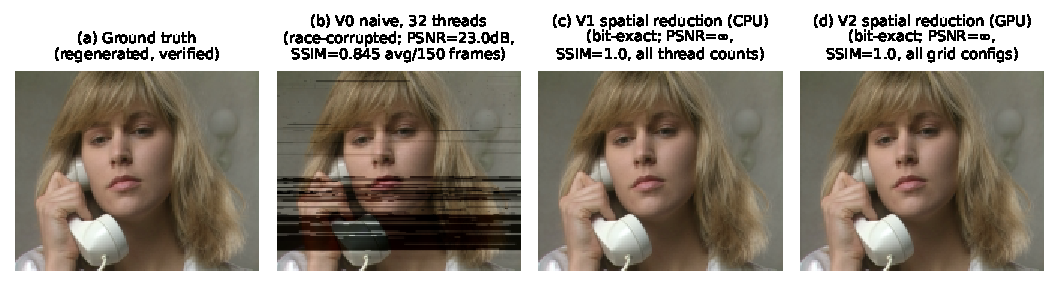
\includegraphics[width=\columnwidth]{figures/correctness_visual_check.pdf}
\caption{Frame 26. Panel (b) adalah satu run V0 representatif dari tiga run -- V0 adalah baseline naif yang murni CPU, tidak ada komputasi GPU yang terlibat. Run ini memakai 32 thread OpenMP pada CPU host Intel i9-14900K milik platform desktop kedua (yang GPU diskretnya tidak dipakai di sini) ($21.5$~dB PSNR-Y / $0.767$ SSIM terhadap (a)); artefak scanline horizontalnya berasal dari penulisan tanpa sinkronisasi ke \texttt{img\_fltr\_8}. Panel (c) dan (d) identik piksel demi piksel dengan (a) pada setiap konfigurasi yang diuji.}
\label{fig:correctness}
\end{figure}

\subsection{Penskalaan Kinerja dan Benchmark Akurasi}

Tabel~\ref{tab:benchmark} menyajikan hasil untuk kedua platform pada berbagai jumlah thread, akurasi, dan konfigurasi grid GPU.

\begin{table*}[htbp]
\caption{Konfigurasi Kunci pada Kedua Platform: Kinerja dan Deviasi terhadap Referensi Deterministik Terverifikasi Masing-Masing Platform. Waktu wall-clock adalah rerata $\pm$ SD atas 6 run terukur dari 7 kali pengulangan.}
\label{tab:benchmark}
\centering
\footnotesize
\setlength{\tabcolsep}{3pt}
\resizebox{\textwidth}{!}{%
\begin{tabular}{llcccccc}
\toprule
Varian & Konfigurasi / Thread & Waktu Wall (ms) & Percepatan vs. Serial & Percepatan vs. CPU Terbaik & Dev. dari Ref. (dB) & SSIM & Kernel L8 GPU (ms) \\
\midrule
\multicolumn{8}{l}{\emph{GB10 (ASUS GX10), memori terpadu; tangga thread CPU 1--20}} \\
CPU V0 (Naif) & 1 Thread & $18{,}240.50 \pm 228.82$ & 1.00$\times$ & T/A & bit-exact & bit-exact & T/A \\
CPU V0 (Naif) & 4 Thread (terburuk) & $7{,}074.33 \pm 90.21$ & 2.58$\times$ & T/A & 13.785 & 0.518246 & T/A \\
CPU V0 (Naif) & 20 Thread (Maks, tercepat) & $6{,}346.33 \pm 32.60$ & 2.87$\times$ & T/A & 25.751 & 0.838930 & T/A \\
CPU V1 (Baseline) & 1 Thread (Serial) & $21{,}552.33 \pm 298.07$ & 1.00$\times$ & T/A & bit-exact & bit-exact & T/A \\
CPU V1 & 4 Thread (bdk. optimum RTX) & $8{,}316.50 \pm 58.06$ & 2.59$\times$ & T/A & bit-exact & bit-exact & T/A \\
CPU V1 (Inti Maks) & 20 Thread (terverifikasi tercepat) & $6{,}921.83 \pm 82.49$ & 3.11$\times$ & T/A & bit-exact & bit-exact & T/A \\
GPU V2 (Hibrida) & Grid $16{\times}16\_256$ (baseline) & $4{,}935.67 \pm 36.30$ & 4.37$\times$ & 1.40$\times$ & bit-exact & bit-exact & $696.51 \pm 1.78$ \\
GPU V2 (Grid Terbaik) & Grid $32{\times}8\_256$ & $4{,}756.33 \pm 30.71$ & 4.53$\times$ & 1.46$\times$ & bit-exact & bit-exact & $533.19 \pm 2.58$ \\
\midrule
\multicolumn{8}{l}{\emph{Desktop RTX 4090, memori diskret; tangga thread CPU 1--32, latar GPU 4 thread}} \\
CPU V0 (Naif) & 1 Thread & $20{,}973.50 \pm 36.30$ & 1.00$\times$ & T/A & bit-exact & bit-exact & T/A \\
CPU V0 (Naif) & 4 Thread (tercepat) & $8{,}207.67 \pm 247.16$ & 2.56$\times$ & T/A & 68.559 & 0.999957 & T/A \\
CPU V0 (Naif) & 32 Thread (Maks, terburuk) & $26{,}388.67 \pm 664.00$ & 0.79$\times$ & T/A & 23.006 & 0.845283 & T/A \\
CPU V1 (Baseline) & 1 Thread (Serial) & $22{,}904.17 \pm 86.90$ & 1.00$\times$ & T/A & bit-exact & bit-exact & T/A \\
CPU V1 (Terbaik) & 4 Thread (terverifikasi tercepat) & $8{,}844.17 \pm 132.68$ & 2.59$\times$ & T/A & bit-exact & bit-exact & T/A \\
GPU V2 (Hibrida) & Grid $16{\times}16\_256$ (baseline) & $5{,}579.00 \pm 166.61$ & 4.11$\times$ & 1.59$\times$ & bit-exact & bit-exact & $437.06 \pm 3.86$ \\
GPU V2 (Grid Terbaik) & Grid $32{\times}8\_256$ & $5{,}435.50 \pm 148.01$ & 4.21$\times$ & 1.63$\times$ & bit-exact & bit-exact & $360.92 \pm 7.22$ \\
\bottomrule
\end{tabular}%
}

\vspace{2mm}
\footnotesize{\emph{Percepatan vs. Serial}: baris CPU dibandingkan terhadap waktu 1 thread variannya sendiri; GPU V2 tidak punya waktu 1 thread, sehingga penyebutnya adalah waktu serial CPU V1 di platform tersebut (Bagian~\ref{sec:gb10-speedup} juga melaporkannya terhadap waktu serial V0 yang lebih cepat dan bit-exact). \emph{Percepatan vs. CPU Terbaik}: hanya untuk GPU V2, terhadap konfigurasi CPU V1 tercepat yang kebenarannya terverifikasi. \emph{Dev./SSIM} diukur terhadap referensi deterministik masing-masing platform; ``bit-exact'' secara logis setara dengan hasil \texttt{cmp -l}, bukan pengukuran kualitas yang berdiri sendiri, dan angkanya adalah rerata seluruh komponen (Bagian~\ref{sec:methodology}). \emph{Kernel L8 GPU}: rerata $\pm$ SD atas 6 run dari sweep profiling (Bagian~\ref{sec:breakdown}); waktu kernel untuk tiga konfigurasi grid sisanya diberikan di Bagian~\ref{sec:warp-generalize}.}
\end{table*}

\subsection{Kualitas Rekonstruksi terhadap Referensi Resolusi Tinggi}
\label{sec:quality}
Karena tidak ada ground truth resolusi tinggi di dalam pipeline, kami membangunnya sendiri: Suzie di-downsample bicubic ke $88{\times}72$, direkonstruksi pada skala 2, lalu dinilai terhadap citra aslinya, dengan upscaling bicubic dari masukan yang sama sebagai pembanding. Kami melaporkan luminansi saja, sebab hanya bidang Y yang melewati jaringan. FSRCNN mencapai $37.86$~dB PSNR-Y dan $0.9665$ SSIM-Y terhadap $35.69$~dB dan $0.9532$ milik bicubic, yakni selisih $2.17$~dB atas 150 frame. Ini satu sekuens pada satu faktor skala, sebuah uji kewajaran dan bukan klaim tentang FSRCNN secara umum~\cite{dong2016fsrcnn}.

\subsection{Biaya Determinisme, Dikuantifikasi}
\label{sec:cost-of-determinism}
Tabel~\ref{tab:benchmark} mengukur biaya di sisi CPU secara langsung, yaitu selisih waktu wall-clock antara V0 (rawan race, tanpa privatisasi) dan V1 (terprivatisasi) pada jumlah thread yang sepadan: $+18.2\%$, $+17.6\%$ dan $+9.1\%$ pada 1, 4 dan 20 thread di GB10, serta $+9.2\%$ dan $+7.8\%$ pada 1 dan 4 thread di RTX 4090. Selisih ini mengisolasi privatisasi, bukan perbedaan seberapa banyak pekerjaan yang di-thread. V0 dan V1 memparalelkan dekonvolusi yang sama, dan tahap reduksi V1 sendiri paralel atas piksel keluaran (Bagian~II-C). Yang diukur selisih itu adalah penulisan dan pembacaan ulang $43.3$~MiB buffer privat, bukan serialisasi sebuah tahap. Determinisme karena itu berbiaya $8$--$18\%$ waktu wall-clock CPU. Titik-titik GB10 mengisyaratkan biayanya menurun begitu mesin jenuh, tetapi 1 dan 4 thread nyaris identik ($18.2\%$ vs. $17.6\%$), sehingga ini paling banter efek dua tingkat, bukan sebuah tren.

Di sisi GPU, instrumentasi per-kernel (Bagian~\ref{sec:breakdown}) menempatkan biaya yang sama dalam satuan yang sebanding. Tahap reduksi adalah padanan overhead privatisasi di GPU, dan ia menyumbang $4.6\%$ jendela event Layer~8 pada GB10 dan $0.6\%$ pada RTX 4090. Porsi itu dihitung terhadap waktu Layer~8, bukan terhadap waktu wall-clock. Bila disetarakan dengan basis $8$--$18\%$ milik CPU, reduksinya hanya menelan $0.55\%$ dan $0.05\%$ waktu ujung ke ujung, dan di situlah besarnya pergeseran itu benar-benar terlihat. Memori device puncak tetap $44.3$~MiB termasuk padding alokator, di bawah $0.1\%$ dari kolam mana pun; kami menyebutnya hasil bandwidth dan paralelisme, bukan kapasitas, karena pada GB10 tidak ada VRAM terpisah yang bisa menjadi tujuan perpindahan buffer. Jarak antara kedua GPU bersifat arsitektural, bukan algoritmik: reduksinya terikat bandwidth dan L2 RTX 4090 menampung seluruh buffer privat. Determinisme secara konstruktif dengan demikian paling murah ketika kapasitas cache melampaui working set privatisasi. Dari situ lahir sebuah kaidah rancangan untuk menerapkan pola ini pada jaringan yang lebih besar: overhead menskala menurut seberapa jauh buffer melampaui last-level cache, bukan menurut jumlah kanal.

\subsection{Rincian Waktu GPU Secara Rinci}
\label{sec:breakdown}
Kami memasang profiling CUDA Event di dalam biner GPU dan menjalankan konfigurasi optimal ($32{\times}8\_256$) enam kali pada tiap platform (Tabel~\ref{tab:breakdown}).

\emph{Mengapa kami tidak melaporkan angka host ke device.} Pencacah sisi host \texttt{h2d\_ms} tidak dapat dibaca sebagai waktu transfer, dan kami mengecualikannya. Salinan-salinan tersebut di-issue \emph{di dalam} jendela yang diukur \texttt{gpu\_l8\_ms}, dan sebuah blocking copy tidak dapat dimulai sebelum kernel yang diluncurkan sebelumnya tuntas, sehingga pencacah itu membebankan waktu menunggu kernel kepada transfer. Sweep-nya memperjelas hal ini: \texttt{h2d\_ms} bergeser $167$~ms pada GB10 ketika yang berubah hanya \emph{bentuk blok kernel}, padahal jumlah byte yang ditransfer identik sepanjang seluruh konfigurasi. Pencacah yang bergerak mengikuti bentuk blok pada jumlah byte tetap bukanlah pencacah yang mengukur byte. Sebagai gantinya kami melaporkan dekomposisi per-kernel.

\begin{table}[htbp]
\caption{Rincian Profiling Layer~8, $32{\times}8\_256$, 150 Frame (ms, rerata $\pm$ SD atas 6 run)}
\label{tab:breakdown}
\centering
\resizebox{\columnwidth}{!}{%
\begin{tabular}{lrr}
\toprule
Tahap Pipeline & GB10 (terpadu) & RTX 4090 (diskret) \\
\midrule
CPU Layer 1--7 & $3{,}392.82 \pm 21.62$ & $4{,}624.50 \pm 70.96$ \\
GPU Layer 8, jendela event & $533.19 \pm 2.58$ & $360.92 \pm 7.22$ \\
\quad$\hookrightarrow$ \texttt{deconv\_kernel} ($56\times$) & $424.07 \pm 0.76$ & $261.90 \pm 3.09$ \\
\quad$\hookrightarrow$ \texttt{spatial\_reduction} ($1\times$) & $26.32 \pm 1.02$ & $2.62 \pm 0.01$ \\
\quad$\hookrightarrow$ transfer dalam jendela, jeda & $127.65 \pm 4.10$ & $152.14 \pm 0.36$ \\
Device ke Host & $3.46 \pm 0.06$ & $16.42 \pm 0.49$ \\
Tak terhitung (launch, I/O berkas) & $821.20$ & $469.33$ \\
\midrule
Total Waktu Wall & $4{,}750.67 \pm 30.40$ & $5{,}471.17 \pm 76.17$ \\
\bottomrule
\end{tabular}%
}

\vspace{1mm}
\footnotesize{Baris berindentasi mendekomposisi jendela event di atasnya dan bukan irisan waktu wall-clock tambahan. Baris-baris itu berasal dari biner terinstrumentasi terpisah yang pencatatan event-nya menggelembungkan jendela tersebut sebesar $8.4\%$ (GB10) dan $15.4\%$ (RTX 4090). Overhead itu terjadi \emph{per launch}, sehingga hampir seluruhnya terkonsentrasi pada $8{,}400$ launch \texttt{deconv\_kernel}, bukan pada $150$ launch reduksi: membagi penggelembungan dengan jumlah launch menghasilkan $5.34$~\textmu s (GB10) dan $6.64$~\textmu s (RTX 4090), dua platform independen yang sepakat dalam orde yang sama. Angka reduksinya karena itu hanya menggelembung sekitar $0.80$~ms pada GB10, sekitar $3\%$, dan mendeflasi seluruh jendela secara seragam justru akan keliru menempatkan reduksi di atas puncak DRAM platformnya. Pencacah produksi \texttt{h2d\_ms} sengaja tidak disertakan (lihat teks).}
\end{table}

Dua hasil menonjol, dan keduanya menunjuk ke arah berlawanan.

Kernel reduksi berbiaya $26.32$~ms pada GB10 tetapi hanya $2.62$~ms pada RTX 4090, jarak $10.0\times$ yang jauh lebih besar daripada keunggulan komputasi umum mana pun (dekonvolusinya hanya berbeda $1.6\times$). Reduksinya murni terikat bandwidth, membaca seluruh buffer privat $43.31$~MiB sekali per frame, yakni $6.81$~GB sepanjang 150 frame: $259$~GB/s pada GB10, sekitar $95\%$ dari puncak $273$~GB/s kolam LPDDR5x-nya~\cite{asusgx10_datasheet}, dan $2{,}597$~GB/s pada RTX 4090, lebih dari $2.5\times$ bandwidth GDDR6X kartu itu yang sebesar $1{,}008$~GB/s. Mengoreksi overhead instrumentasi per-launch (Tabel~\ref{tab:breakdown}) menggeser angka GB10 ke $267$~GB/s, tetap di bawah puncak, dan mendorong angka RTX 4090 makin jauh di atas puncaknya sendiri. Working set yang berada di DRAM tidak mungkin menghasilkan angka seperti itu. Penjelasan yang wajar adalah L2 $72$~MB milik RTX 4090, yang cukup untuk menampung buffer tersebut, sehingga reduksinya sebagian besar dilayani dari cache sementara GB10 harus melakukan streaming dari memori terpadu mendekati puncak perangkat kerasnya. Kami menyodorkan ini sebagai pembacaan yang paling konsisten dengan bandwidth terukur, bukan sebagai fakta hasil profiling, sebab kami tidak merekam pencacah L2 (Bagian~\ref{sec:limitations}).

Transfer device ke host berjalan ke arah sebaliknya: $3.46$~ms berbanding $16.42$~ms, keunggulan $4.74\times$ bagi memori terpadu pada muatan yang identik ($35.1$ vs. $7.4$~GB/s efektif). Inilah kontras memori terpadu versus diskret yang paling bersih dalam data kami, dan tidak seperti \texttt{h2d\_ms}, pengukurannya berada di luar jendela event, setelah \texttt{cudaEventSynchronize}, tanpa eksekusi kernel yang bisa mencampurinya.

Memori device puncak tetap terbatas pada $45{,}382$~KiB ($\approx44.3$~MiB) di kedua platform pada setiap konfigurasi, sekitar 1~MiB di atas minimum teoretis $43.3$~MiB (Bagian~II-C).

%%%%%%%%%%%%%%%%%%%%%%%%%%%%%%%%%%%%%%%%%%%%%%%%%%%%%%%%%%%%%%%%%%%%%%%%%%%%%%%
\section{Pembahasan dan Temuan Utama}

\subsection{Percepatan terhadap CPU Berinti Penuh, dan Penyelarasan Warp}
\label{sec:gb10-speedup}
Kami melaporkan percepatan terhadap CPU V1, bukan V0, pada konfigurasi multi-thread: V1 bebas race pada setiap jumlah thread, sedangkan V0 hanya benar secara \emph{kebetulan} pada 1 thread dan memburuk setelahnya. V0 sebenarnya pemenang waktu wall-clock mentah pada 20 thread ($6{,}346.33$~ms, yang hanya akan memberi $1.33\times$), tetapi keluarannya di titik itu tidak terverifikasi benar; kami menyebutkan angkanya ketimbang menghilangkannya. GPU V2 ($32{\times}8\_256$) mencapai $4{,}756.33$~ms ($31.5$ FPS), percepatan $1.46\times$ atas konfigurasi 20 thread CPU V1 ($6{,}921.83$~ms, hasil CPU tercepat yang kebenarannya terverifikasi).

Perbandingan serial menuntut kehati-hatian lebih, sebab kedua varian tidak berbagi baseline serial. Pada 1 thread V0 bersifat bit-exact sekaligus lebih cepat daripada V1 ($18{,}240.50$ vs. $21{,}552.33$~ms) karena ia melewati privatisasi yang dibayar V1, dan itu menjadikannya baseline serial \emph{bit-exact} tercepat yang tersedia: $3.84\times$ (GB10) dan $3.86\times$ (RTX 4090). Terhadap waktu serial V1, angkanya naik ke $4.53\times$ dan $4.21\times$, digelembungkan oleh penyebut yang lebih lambat, sehingga kami mengedepankan $3.84\times$. Baseline-nya bukan lawan yang lemah: inferensi CNN menskala baik pada klaster ARM big.LITTLE bila dijadwalkan dengan benar~\cite{wang2020pipeit}, dan inti-inti GB10 menskala mulus di sepanjang tangga thread tanpa keruntuhan seperti yang ditunjukkan RTX 4090 di atas 8 thread. GPU V2 juga konfigurasi yang paling stabil ($\pm30.71$ berbanding $\pm82.49$~ms).

Beralih dari grid default $16{\times}16$ ($696.51 \pm 1.78$~ms) ke grid selaras warp $32{\times}8$ ($533.19 \pm 2.58$~ms) memangkas waktu kernel $23.4\%$, jarak yang jauh di luar variasi antar-run (SD $1.78$ dan $2.58$~ms). Kami mengaitkannya dengan coalescing: blok selebar 32 thread membuat setiap thread dalam satu warp menerbitkan permintaan ke dalam satu transaksi, sedangkan blok selebar 16 memecahnya ke beberapa transaksi. Rincian per-kernel menguji hal ini lebih tajam daripada yang bisa dilakukan waktu wall-clock. Bentuk blok hanya memengaruhi \texttt{deconv\_kernel}, sebab reduksinya diluncurkan satu dimensi. Jika coalescing memang mekanismenya, seluruh perolehan mestinya jatuh pada dekonvolusi. Dan memang demikian: \texttt{deconv\_kernel} turun $24.9\%$ ($564.74$ ke $424.07$~ms) sementara reduksinya bergerak $+0.9\%$ ($26.08$ ke $26.32$~ms), masih di dalam sebarannya sendiri. Ini tetap inferensi dari waktu, bukan pengukuran langsung efisiensi muat (Bagian~\ref{sec:limitations}).

\subsection{Biaya Transfer dan Hukum Amdahl}
\label{sec:nvlink}
Dibatasi dari atas, transfer bukanlah bottleneck pada kedua platform. Pada GB10, seluruh isi jendela event yang bukan eksekusi kernel berjumlah $127.65$~ms, yakni $2.7\%$ waktu wall-clock, ditambah $3.46$~ms D2H; bahkan bila seluruh residu itu dibebankan sebagai transfer, yang jelas melebih-lebihkan, porsinya tetap di bawah $3\%$ pipeline. Residu RTX 4090 lebih besar baik secara absolut maupun sebagai porsi jendelanya ($152.14$~ms, $36.5\%$ berbanding $22.1\%$), arah yang memang diprediksi PCIe versus NVLink-C2C, meski selisihnya cukup kecil sehingga kami tidak bertumpu padanya. Satu-satunya pengukuran transfer yang bersih sekaligus jelas asimetris adalah D2H.

Yang justru ditunjukkan Tabel~\ref{tab:breakdown} adalah langit-langit Hukum Amdahl~\cite{amdahl1967}. Layer~8 kini tinggal $11.2\%$ waktu wall-clock GB10 dan $6.6\%$ pada RTX 4090, sementara CPU Layer 1--7, yang masih berjalan pada 20 dan 4 thread OpenMP alih-alih serial, menyumbang $71.4\%$ dan $84.5\%$. Menggratiskan Layer~8 pun masih menyisakan pipeline RTX 4090 pada $93\%$ waktu wall-clock saat ini, sehingga memindahkan Layer 1--7 adalah satu-satunya jalan tersisa menuju rekonstruksi di bawah satu detik; analisis Roofline~\cite{williams2009roofline} akan memastikan lebih dulu apakah pemindahan itu terikat komputasi atau memori. Sisa yang tak terhitung adalah peluncuran proses, I/O berkas dan konversi \texttt{uint8}$\leftrightarrow$\texttt{double} per frame, yang semuanya berjalan satu thread dan berada di luar wilayah terinstrumentasi.

%%%%%%%%%%%%%%%%%%%%%%%%%%%%%%%%%%%%%%%%%%%%%%%%%%%%%%%%%%%%%%%%%%%%%%%%%%%%%%%
\section{Validasi Lintas Platform pada Perangkat Keras GPU Diskret}
\label{sec:rtx4090}

Untuk menguji apakah pendekatan ini berlaku umum di luar memori terpadu, kami mereplikasi eksperimennya pada desktop ber-GPU diskret (Tabel~\ref{tab:hardware}). Dua perbedaan penting: memori CPU dan GPU terpisah melalui PCIe alih-alih berbagi satu kolam, dan CPU-nya heterogen (24 thread fisik / 32 logis pada P-core dan E-core) berhadapan dengan 20 inti homogen per tingkat milik GB10 yang tanpa SMT.

\subsection{Penyesuaian Metodologi dan Percepatan GPU}
Memakai ulang tangga thread GB10 beserta latar 20 thread justru menyesatkan di sini: waktu wall-clock runtuh di atas 8 thread hingga $\sim$3.5$\times$ lebih lambat daripada optimum 4 thread, dan itu berulang pada tiga run penuh. Karena itu kami menyapu tangga yang sesuai topologi (1--32) dan memakai konfigurasi CPU terbaik platform ini sendiri (4 thread) sebagai latar. Keruntuhan itu konsisten dengan pembagian P/E-core yang bertumpu pada Intel Thread Director sementara kolam OpenMP generik tidak membawa kendali afinitas~\cite{eichenberger2012ompaffinity}, meski optimum 4 thread tidak cocok rapi dengan 8 P-core, sehingga kami tidak mengklaim penjelasan yang terkonfirmasi (Bagian~\ref{sec:limitations}). Hal ini insidental terhadap kontribusi kami, dan kami laporkan karena ia mengubah apa yang pantas disebut baseline CPU yang adil di sini. Dengan latar yang sudah dikoreksi, GPU V2 mencapai $5{,}435$--$5{,}579$~ms ($26.9$--$27.6$ FPS), yakni $1.59\times$--$1.63\times$ atas CPU V1 terbaik (4 thread, $8{,}844.17$~ms). Angka itu bukan $4\times$+ yang menggelembung karena dibandingkan terhadap waktu serial, atau terhadap run berjumlah thread tinggi yang sudah runtuh seperti CPU V0 pada 32 thread (Tabel~\ref{tab:benchmark}).

\subsection{Kesamaan Bit Lintas Arsitektur}
\label{sec:cross-arch-bitexact}
Bagian~\ref{sec:methodology} menegakkan bit-exactness \emph{di dalam} tiap platform. Apakah keluaran GPU V2 identik \emph{antar} keduanya merupakan pertanyaan yang lebih kuat. GB10 (host ARM, \texttt{sm\_121}) dan RTX 4090 (host x86, \texttt{sm\_89}) berbeda dalam ISA host dan mikroarsitektur GPU, sehingga keluaran identik-bit tidak dijamin hanya oleh kepatuhan IEEE-754 \texttt{double}: pembangkitan kode untuk dua target SM, kontraksi FMA, dan pustaka matematika masing-masing bisa menyimpang pada bit terakhir. Rantai perkakasnya di luar itu tergolong seragam (GCC 13.3.0 dan CUDA 13.0 pada keduanya), sehingga uji ini mengisolasi ISA dan mikroarsitektur alih-alih menumpuknya dengan perbedaan toolkit; klaim lintas-\emph{toolkit} memerlukan eksperimennya sendiri. Menjalankan konfigurasi pemenang $32{\times}8$ pada keduanya, \texttt{cmp -l} melaporkan $0$ byte berbeda dan digest SHA-256 keduanya cocok (\texttt{8db2c07a...ca066b}). Itulah bentuk terkuat dari klaim determinisme yang diajukan makalah ini.

\subsection{Penyelarasan Warp Berlaku Umum Lintas Arsitektur GPU}
\label{sec:warp-generalize}
Pada tingkat kernel, $32{\times}8$ tetap tercepat di GPU Ada Lovelace ini ($360.92 \pm 7.22$~ms), $17.4\%$ lebih cepat daripada $16{\times}16$ ($437.06 \pm 3.86$~ms), yang menegaskan bahwa argumen coalescing pada Bagian~III-B, sebagai konsekuensi granularitas warp 32 thread milik CUDA~\cite{nvidiacudaguide}, merupakan sifat CUDA dan bukan sifat khas GB10. Pelokalannya pun bertahan: \texttt{deconv\_kernel} turun $15.6\%$ ($310.32$ ke $261.90$~ms) sementara reduksinya tak berubah di $2.62$~ms. Gbr.~\ref{fig:warp-cross} membandingkan kelima konfigurasi grid pada kedua GPU, lengkap dengan error bar atas enam run. Pada tingkat \emph{wall-clock}, kelimanya sulit dibedakan secara statistik ($5{,}435$--$5{,}579$~ms, error bar-nya bertumpang tindih) meski $32{\times}8$ secara nominal unggul di kedua metrik; keunggulan tingkat kernelnya hanya terlihat lewat profiling CUDA Event, dan itulah sebabnya instrumentasi tersebut penting.

\begin{figure}[htbp]
\centering
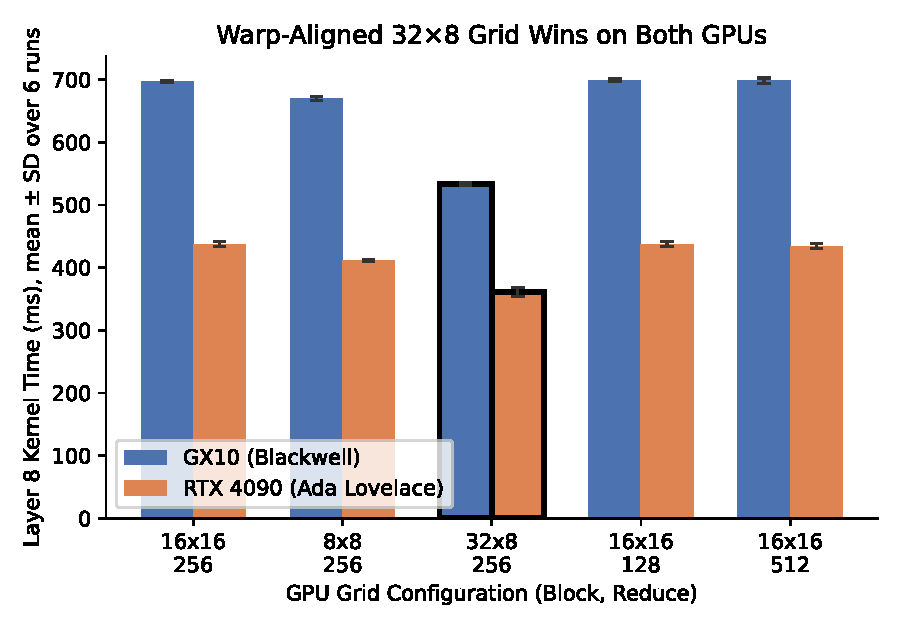
\includegraphics[width=\columnwidth]{figures/warp_alignment_cross_platform.pdf}
\caption{Waktu kernel Layer~8 GPU menurut konfigurasi grid, rerata $\pm$ SD atas 6 run. Grid selaras warp $32{\times}8$ (bergaris tebal) tercepat pada kedua arsitektur.}
\label{fig:warp-cross}
\end{figure}

\subsection{Memori Non-Terpadu dan Presisi FP64}
Memori CPU dan GPU di sini terpisah secara fisik melalui PCIe, tidak seperti kolam terpadu GB10~\cite{nvidiagracehopper2022,wahlgren2025upm}. Meski begitu, kernel Layer~8 platform inilah yang lebih cepat di antara keduanya. Tabel~\ref{tab:breakdown} mengaitkannya dengan keunggulan komputasi dan cache pada Bagian~\ref{sec:breakdown}, bukan dengan absennya biaya transfer: overhead PCIe/DMA~\cite{go2017apunet} jelas terlihat pada residu dan angka D2H, tetapi ia kalah bobot. Karena itu kami memperkirakan keseimbangannya bergeser begitu working set melampaui L2 kartu ini. Presisi ganda juga menuntut harga di sini. Throughput FP64-nya secara arsitektural $1/64$ dari FP32, sehingga waktu kernel di atas dicapai dengan sumber daya komputasi dominannya menganggur, dan port FP32 sangat mungkin jauh lebih cepat dengan konsekuensi melemahnya bit-exactness menjadi sekadar toleransi numerik.

%%%%%%%%%%%%%%%%%%%%%%%%%%%%%%%%%%%%%%%%%%%%%%%%%%%%%%%%%%%%%%%%%%%%%%%%%%%%%%%
\section{Keterbatasan dan Pekerjaan Lanjutan}
\label{sec:limitations}
Celah terbesarnya adalah tidak adanya baseline GPU pembanding: V2 hanya diadu dengan implementasi CPU, bukan dengan \texttt{atomicAdd}, kernel gather output-stationary, atau cuDNN. Dua penjelasan kami merupakan inferensi dari waktu, bukan pengukuran langsung. Penjelasan berbasis cache atas jarak $10\times$ pada reduksi akan tuntas bila ada pencacah hit-rate L2 dan sapuan working set melintasi batas L2; penjelasan coalescing, meski sudah terlokalisasi pada \texttt{deconv\_kernel} sesuai prediksi, akan tuntas bila ada pencacah efisiensi muat dan lebar blok yang tidak selaras. Angka host ke device kami juga masih berupa batas atas yang memuat overhead peluncuran dan padding sisi host, yang dapat dipisahkan dengan pinned memory atau beberapa stream, meski D2H tidak terpengaruh. Tidak ada ablasi FP32 yang mengukur pertukaran antara percepatan dan bit-exactness, dan tidak ada eksperimen kendali \texttt{OMP\_PROC\_BIND} yang mengisolasi keruntuhan RTX 4090 dari kejenuhan bandwidth atau throttling termal. Terakhir, seluruh hasil memakai satu sekuens QCIF ke CIF sepanjang 150 frame, dengan kualitas rekonstruksi (Bagian~\ref{sec:quality}) diukur pada satu faktor skala terhadap pengganti hasil downsample bicubic, dan kroma direplikasi alih-alih direkonstruksi. Resolusi yang lebih tinggi akan menggeser rasio komputasi terhadap transfer dan mendorong buffer privat melewati L2 RTX 4090, yakni rezim yang paling menguji kaidah rancangan kami.

%%%%%%%%%%%%%%%%%%%%%%%%%%%%%%%%%%%%%%%%%%%%%%%%%%%%%%%%%%%%%%%%%%%%%%%%%%%%%%%
\section{Kesimpulan}
Kami memperkenalkan kerangka reduksi spasial GPU untuk dekonvolusi Layer~8 FSRCNN dan mengevaluasinya pada dua platform yang berbeda secara arsitektural. Pada keduanya, varian CPU maupun GPU bersifat bit-exact terhadap referensi deterministik terverifikasi di setiap konfigurasi yang diuji, sementara akumulasi naif merusak keluaran secara tidak monoton, turun serendah $13.8$~dB dan mencapai $68.6$~dB yang nyaris tak terdeteksi, kegagalan yang justru lebih instruktif. Keluaran GPU bahkan identik-bit \emph{antar} kedua platform, mencakup dua ISA host dan dua generasi GPU. Grid selaras warp $32{\times}8$ tercepat pada keduanya, dengan profiling per-kernel yang melokalisasi seluruh perolehan pada dekonvolusi sebagaimana dituntut penjelasan coalescing, dan percepatan terhadap konfigurasi CPU terbaik yang kebenarannya terverifikasi mencapai $1.46\times$ ($31.5$ FPS) dan $1.63\times$. Kedua asimetri platform berjalan ke arah berlawanan. Memori terpadu mengembalikan hasil $4.74\times$ lebih cepat, sedangkan GPU diskret menjalankan reduksi yang terikat bandwidth $10.0\times$ lebih cepat karena L2-nya menampung seluruh buffer privat yang harus di-streaming GB10 pada $95\%$ puncak memorinya. Biaya determinisme dengan demikian lebih bergantung pada apakah working set privatisasi muat di last-level cache daripada pada algoritmanya, sebuah batas yang semestinya berlaku pula untuk jaringan mana pun yang menerapkan pola ini.

%%%%%%%%%%%%%%%%%%%%%%%%%%%%%%%%%%%%%%%%%%%%%%%%%%%%%%%%%%%%%%%%%%%%%%%%%%%%%%%
\begin{thebibliography}{00}
\footnotesize
\itemsep0pt plus 0.5pt

\bibitem{annisa2025} Annisa, Adnan, and Z. Zainuddin, ``Enhancing computational efficiency: transitioning from serial to parallel programming for low-to-high resolution video reconstruction using FSRCNN on AMP architecture,'' in \emph{Proc. IEEE Int. Conf. Artif. Intell. Mechatron. Syst. (AIMS)}, 2025, pp. 1--8.

\bibitem{dong2016fsrcnn} C. Dong, C. C. Loy, and X. Tang, ``Accelerating the super-resolution convolutional neural network,'' in \emph{Proc. ECCV}, 2016, pp. 391--407.

\bibitem{wang2020pipeit} S. Wang \emph{et al.}, ``High-throughput CNN inference on embedded ARM big.LITTLE multicore processors,'' \emph{IEEE TCAD}, vol. 39, no. 10, pp. 2254--2267, 2020.

\bibitem{bilbao2023pmcsched} C. Bilbao, J. C. Saez, and M. Prieto-Mat\'ias, ``Flexible system software scheduling for asymmetric multicore systems with PMCSched: a case for Intel Alder Lake,'' \emph{Concurr. Comput. Pract. Exper.}, vol. 35, no. 25, e7814, 2023.

\bibitem{eichenberger2012ompaffinity} A. E. Eichenberger \emph{et al.}, ``The design of OpenMP thread affinity,'' in \emph{IWOMP}, LNCS 7312, 2012, pp. 15--28.

\bibitem{nvidiacudaguide} NVIDIA Corp., \emph{CUDA C++ Programming Guide}. [Online]. Available: docs.nvidia.com/cuda/cuda-c-programming-guide/

\bibitem{go2017apunet} Y. Go \emph{et al.}, ``APUNet: revitalizing GPU as packet processing accelerator,'' in \emph{Proc. USENIX NSDI}, 2017, pp. 83--96.

\bibitem{wang2004ssim} Z. Wang \emph{et al.}, ``Image quality assessment: from error visibility to structural similarity,'' \emph{IEEE Trans. Image Process.}, vol. 13, no. 4, pp. 600--612, 2004.

\bibitem{dong2014srcnn} C. Dong \emph{et al.}, ``Learning a deep convolutional network for image super-resolution,'' in \emph{Proc. ECCV}, 2014, pp. 184--199.

\bibitem{amdahl1967} G. M. Amdahl, ``Validity of the single processor approach to achieving large scale computing capabilities,'' in \emph{Proc. AFIPS}, 1967, pp. 483--485.

\bibitem{williams2009roofline} S. Williams, A. Waterman, and D. Patterson, ``Roofline: an insightful visual performance model for multicore architectures,'' \emph{Commun. ACM}, vol. 52, no. 4, pp. 65--76, 2009.

\bibitem{chetlur2014cudnn} S. Chetlur \emph{et al.}, ``cuDNN: efficient primitives for deep learning,'' arXiv:1410.0759, 2014.

\bibitem{serebryany2009threadsanitizer} K. Serebryany and T. Iskhodzhanov, ``ThreadSanitizer: data race detection in practice,'' in \emph{Proc. WBIA}, 2009, pp. 62--71.

\bibitem{lashgar2012warpresize} A. Lashgar, A. Baniasadi, and A. Khonsari, ``Warp size impact in GPUs: large or small?,'' in \emph{Proc. GPGPU-5}, 2012, pp. 27--32.

\bibitem{dumoulin2016convolution} V. Dumoulin and F. Visin, ``A guide to convolution arithmetic for deep learning,'' arXiv:1603.07285, 2016.

\bibitem{nvidiagb10_2025} NVIDIA Corp., ``NVIDIA puts Grace Blackwell on every desk and at every AI developer's fingertips,'' NVIDIA Newsroom, Jan. 2025. [Online]. Available: nvidianews.nvidia.com/news/nvidia-puts-grace-blackwell-on-every-desk-and-at-every-ai-developers-fingertips

\bibitem{asusgx10_datasheet} ASUSTeK Computer Inc., \emph{ASUS Ascent GX10 Datasheet}, v8, 2025. [Online]. Available: dlcdnwebimgs.asus.com/files/media/202506/5c0fb57c-4e48-4e96-8c97-04bf8df2677c/asus-ascent-gx10-datasheet.pdf

\bibitem{armdynamiq} Arm Ltd., ``DynamIQ technology.'' [Online]. Available: arm.com/technologies/dynamiq

\bibitem{nvidiaada2022} NVIDIA Corp., \emph{NVIDIA Ada GPU Architecture}, Whitepaper V2.02, 2022.

\bibitem{nvidiagracehopper2022} NVIDIA Corp., ``Grace Hopper Superchip architecture in-depth,'' NVIDIA Developer Blog, 2022.

\bibitem{wahlgren2025upm} J. Wahlgren \emph{et al.}, ``Dissecting CPU-GPU unified physical memory on AMD MI300A APUs,'' in \emph{Proc. IEEE IISWC}, 2025.

\end{thebibliography}

\end{document}

%%%%%%%%%%%%%%%%%%%%%%%%%%%%%%%%%%%%%%%%%%%%%%%%%%%%%%%%%%%%%%%%%%%%%%%%%%%%%%%
% CATATAN INTERNAL -- BUKAN BAGIAN DARI PAPER.
% Semua yang di bawah ini berada SETELAH \end{document}, jadi tidak pernah
% ikut di-compile atau muncul di PDF. Ini murni catatan pribadi untuk
% memvalidasi bahwa setiap angka di naskah di atas benar-benar berasal dari
% hasil eksperimen (bukan karangan), lengkap dengan path file mentahnya.
% Jangan dihapus otomatis oleh tooling BibTeX/pdflatex -- aman, karena TeX
% berhenti memproses begitu menemui \end{document}.
%%%%%%%%%%%%%%%%%%%%%%%%%%%%%%%%%%%%%%%%%%%%%%%%%%%%%%%%%%%%%%%%%%%%%%%%%%%%%%%

===============================================================================
PETA SUMBER DATA -- itis_id.tex
===============================================================================
Semua file mentah ada di plans/ (bukan di sync-pilot/, itu proyek scheduler
yang beda). Indeks resmi skrip -> output: plans/COLLECT_README.md, baca itu
dulu. Ringkasan per bagian paper di bawah.

-------------------------------------------------------------------------------
1. Tabel Hardware (tab:hardware, baris ~119-141)
-------------------------------------------------------------------------------
Sumber : plans/results_env_gb10.txt, plans/results_env_rtx4090.txt
Dari   : plans/collect_env.sh

  - GB10   : CUDA 13.0, V13.0.88, Driver 580.159.03 -> cocok baris 135.
  - RTX4090: CUDA 13.0, V13.0.48, Driver 580.65.06, compute_cap 8.9
             -> cocok baris 135 & label sm_89 di baris 131.
  - CPU model (Cortex-X925/A725, i9-14900K), jumlah core, cache, RAM:
    semua dari output lscpu/free -h di file yang sama.

  CATATAN VALIDASI: hostname GB10 tercatat "node6". COLLECT_README.md
  (baris 26-33) sempat curiga node6 BUKAN mesin GB10 asli, karena file lama
  results/spesifikasi/75-gcc-nvcc.txt melaporkan CUDA 12.0 dari host itu.
  File results_env_gb10.txt yang dipakai sekarang menunjukkan CUDA 13.0 --
  versi yang sudah dikoreksi/diverifikasi ulang. Kalau mau benar-benar
  yakin, bandingkan timestamp kedua file itu.

-------------------------------------------------------------------------------
2. Tabel I -- Performa & Akurasi (tab:benchmark, baris ~178-213)
-------------------------------------------------------------------------------
GB10 (baris CPU V0/V1) : results/gpu-4.txt baris 327-340
  Cocok persis: 18240.50+-228.82 | 7074.33+-90.21 | 6346.33+-32.60 |
                21552.33+-298.07 | 8316.50+-58.06 | 6921.83+-82.49

RTX4090 (semua baris V0/V1/V2) : plans/raw_results.csv
  Cocok kolom per kolom: wall_ms_mean, wall_ms_sd, psnr_db, ssim, vram_kb.

  !! ADA FILE JEBAKAN: plans/raw_results_v1.csv -- angkanya BEDA dan TIDAK
     cocok tabel (mis. 21631.00+-173.28, bukan 20973.50+-36.30), dan
     diff_bytes-nya rusak (98% byte beda bahkan di V1 1-thread yang
     seharusnya bit-exact). Kelihatan seperti hasil run gagal/lama yang
     TIDAK dipakai di paper final. Jangan tertukar dengan raw_results.csv.

-------------------------------------------------------------------------------
3. Kualitas Rekonstruksi (sec:quality, baris ~217)
-------------------------------------------------------------------------------
Sumber : plans/results_quality_rtx4090.txt
Dari   : plans/collect_reconstruction_quality.sh

  Protokol: Suzie 176x144 (suzie_qcif.yuv) di-downsample bicubic ffmpeg ke
  88x72 (=176/2 x 144/2, sesuai scale factor FSRCNN 2x), lalu direkonstruksi
  balik ke 176x144 oleh FSRCNN dan dibandingkan PSNR/SSIM (plane Y saja)
  terhadap suzie_qcif.yuv ASLI (yang sekarang jadi ground truth valid karena
  kita sendiri yang mengecilkannya). Pembanding kedua: bicubic upscale dari
  88x72 yang sama (baseline "gratis" tanpa neural network).

  Angka baris 20 & 24 file: FSRCNN PSNR y:37.864571 SSIM Y:0.966542
                            Bicubic PSNR y:35.690343 SSIM Y:0.953247
  -> cocok persis dengan "37.86 dB/0.9665 vs 35.69 dB/0.9532" di baris 217.

  Kenapa eksperimen ini ada sama sekali: sebelumnya SEMUA angka kualitas di
  paper cuma bukti self-consistency (V2 GPU vs V1 CPU, makanya "bit-exact"/
  PSNR=inf) -- itu cuma membuktikan port GPU-nya setia meniru CPU, BUKAN
  bukti FSRCNN benar-benar merekonstruksi sesuatu yang berguna. Section ini
  menutup celah itu dengan ground truth buatan sendiri (lihat
  reviews/03.md bagian C untuk kritik aslinya).

  Dijalankan cuma di RTX 4090 (bukan GB10) karena V2 bit-exact di kedua
  platform -- hasil kualitasnya otomatis identik, run ulang di GB10 hanya
  buang waktu.

-------------------------------------------------------------------------------
4. Biaya Determinisme (sec:cost-of-determinism, baris ~221)
-------------------------------------------------------------------------------
BUKAN pengukuran terpisah -- murni aritmetika delta dari Tabel I di atas
(V1 - V0) / V0 pada thread count yang sama:

  GB10   1 thread : (21552.33-18240.50)/18240.50 = +18.2%
  GB10   4 thread : (8316.50-7074.33)/7074.33     = +17.6%
  GB10  20 thread : (6921.83-6346.33)/6346.33     = +9.1%
  RTX    1 thread : (22904.17-20973.50)/20973.50  = +9.2%
  RTX    4 thread : (8844.17-8207.67)/8207.67     = +7.8%

Rentang "8--18%" yang dikutip 3x di paper (baris 99 Pendahuluan, baris 221,
baris 223) itu cuma min(7.8%)~8% dan max(18.2%)~18% dari kelima angka di
atas -- bukan tiga eksperimen berbeda, cuma dipakai ulang sebagai ringkasan.

-------------------------------------------------------------------------------
5. Tabel II -- Rincian Profiling Layer 8 (tab:breakdown, baris ~231-255)
-------------------------------------------------------------------------------
GB10    : plans/results_gpuprofile_gb10.txt baris 20 & 31
  Fase A (wall/window)  : 4750.67+-30.40 | 533.19+-2.58 | 3392.82+-21.62
  Fase B (dekomposisi)  : 424.07+-0.76 | 26.32+-1.02 | 127.65+-4.10

RTX4090 : plans/results_gpuprofile_rtx4090.txt baris 20 & 31
  Fase A : 5471.17+-76.17 | 360.92+-7.22 | 4624.50+-70.96
  Fase B : 261.90+-3.09 | 2.62+-0.01 | 152.14+-0.36

Dari plans/collect_gpu_profile.sh (COLLECT_README.md bagian 2):
  - Fase A pakai binary produksi (fsrcnn_gpu_main.cu) -- ini angka resmi
    paper untuk wall time & window gpu_l8.
  - Fase B pakai fsrcnn_gpu_instrumented.cu -- HANYA untuk memecah
    deconv_kernel vs spatial_reduction, bukan pengganti angka Fase A
    (instrumentasinya sendiri menggelembungkan window ~8.4%/15.4%, sudah
    dicatat di footnote Tabel II baris 254).

-------------------------------------------------------------------------------
6. Bandwidth reduksi (259 GB/s GB10, 2597 GB/s RTX4090, baris ~259)
-------------------------------------------------------------------------------
Turunan aritmetika, bukan file terpisah:
  43.31 MiB (buffer privat) x 150 frame / waktu kernel reduksi
  (26.32 ms GB10 atau 2.62 ms RTX4090, dari Tabel II di atas)
Bisa dihitung ulang manual dari angka Tabel II.

-------------------------------------------------------------------------------
7. Kesamaan bit lintas platform (sec:cross-arch-bitexact, baris ~293)
-------------------------------------------------------------------------------
Sumber : plans/gb10_v2_output.yuv.sha256, plans/rtx4090_v2_output.yuv.sha256
Dari   : plans/crossplatform_bitexact_check_gb10.sh /
         plans/crossplatform_bitexact_check_rtx4090.sh

  Sudah dicek langsung -- digest kedua file IDENTIK:
  8db2c07a293e631c1bc033ca5553c615af3cd125a4cb9617d979c2f61aca066b
  -> cocok persis kutipan "8db2c07a...ca066b" di baris 293.

-------------------------------------------------------------------------------
8. Fig. 1 panel (b) -- frame korup V0 (baris ~165-172)
-------------------------------------------------------------------------------
Sumber : plans/results_v0frame_rtx4090.txt
Dari   : plans/collect_v0_frame26.sh

  Tiga run V0 32-thread berbeda (karena race, memang tidak reproducible):
    run 1: diff_bytes=5010476/22809600, PSNR-Y 21.457, SSIM-Y 0.767
    run 2: diff_bytes=5042223/22809600, PSNR-Y 21.633, SSIM-Y 0.777
    run 3: diff_bytes=4749465/22809600, PSNR-Y 21.339, SSIM-Y 0.779
  Paper mengutip run 1 (21.5 dB/0.767) sebagai "representative run" di
  caption Gbr. 1 (baris 170) -- konsisten dengan angka "13.8 dB"/"68.6 dB"/
  "23.0 dB" dan "4.75/5.01/5.04 juta byte" di baris 165, yang sumbernya
  gabungan file ini + plans/raw_results.csv (baris V0 4-thread & 32-thread).
  PNG-nya: plans/v0_frames_rtx4090/*.png.

  Alasan skrip ini dibuat: sebelumnya tidak jelas mesin mana yang
  menghasilkan gambar frame korup di Gbr. 1 -- teks lama sempat menyebutnya
  "GB10 case" padahal angkanya (23.0 dB) justru match baris 32-thread RTX
  4090 di results/76-rtx4090v3.txt:333. COLLECT_README.md bagian 4
  menjelaskan kebingungan ini dan kenapa perlu di-regenerate dengan
  identitas mesin tercetak di output (bukan menebak).

===============================================================================
CARA VALIDASI CEPAT
===============================================================================
1. Buka plans/COLLECT_README.md dulu sebagai peta skrip->output.
2. Untuk tiap angka di paper, grep angka itu di folder plans/ dan results/ --
   hampir semua traceable ke satu file txt/csv mentah seperti di atas.
3. Waspadai file "v1"/"lama" yang mirip nama tapi angkanya beda
   (raw_results_v1.csv, results/spesifikasi/75-gcc-nvcc.txt) -- itu jejak
   iterasi sebelumnya yang sudah digantikan, bukan sumber aktif.
